\documentclass[sigconf]{acmart}

\usepackage{hyperref}

%\usepackage{endfloat}
%\renewcommand{\efloatseparator}{\mbox{}} % no new page between figures

\usepackage{booktabs} % For formal tables

\settopmatter{printacmref=false} % Removes citation information below abstract
\renewcommand\footnotetextcopyrightpermission[1]{} % removes footnote with conference information in first column
\pagestyle{plain} % removes running headers


\begin{document}
\title{Big Data Application in Web Search and Text Mining}


\author{Wenxuan Han}
% \orcid{1234-5678-9012}
\affiliation{%
  \institution{Indiana University Bloomington}
  \streetaddress{1150 S Clarizz Blvd}
  \city{Bloomington} 
  \state{Indiana} 
  \postcode{47401-4294}
}
\email{wenxhan@iu.edu}

% The default list of authors is too long for headers}
% \renewcommand{\shortauthors}{B. Trovato et al.}


\begin{abstract}
Because of the rapid development of social media, there are gigantic amount of data generated in every second on the web. And those data could be stored in any forms like text, videos, images or their combinations. The more complicated forms of data, the more space it will take up and will cost more time to read it. Although most of today's personal computers have a very high performance, it is extremely difficult to process and analyze useful text information from those huge amount of unstructured data by using traditional single computer methods without the help of big data tools or text mining techniques. Fortunately, the improvements in big data application are also increasing fast in order to support those difficult works on web search and text mining. This paper first studies the knowledge of web search technique and its data analytic steps, then introduces the link structure with a broad analysis of some web page structures (Hubs and PageRank), and at last, discusses their applications in this field of big data.
\end{abstract}

\keywords{I523, HID209, Big Data, Social Media, Web Search, Text Mining, PageRank, Hubs}


\maketitle

\section{Introduction}

In recent years, social media has become more and more popular as a new way of communication and knowledge transfer. People could use it to create, share, exchange information and create their own network. Social media usage has been boosted from 2005 to 2015. Users between 18 and 29 ages are the mainly part of social media users \cite{editor01}. Today 90\% of young adults are active on social media. This proportion was 12\% in 2005 \cite{editor02}. And since the development of mobile products, social media has also been offered a better platform for users to share data faster and more convenient. Thus, this proportion could be keep stable or still increase during the next few years.

Nowadays, a growing number of people prefer to express their opinion and feelings through tweeting, sharing images, commenting on social sites \cite{editor01}. Since the amount of such data become extremely large, it is significant to extract and analyze useful information through them by using text analysis methods. Therefore, some applications which based on these information have been developed, such as recommendation system and search engine.

However, as the big data began to appear in the website, there are some problems that people must face for web search which include the longer search queries (key words) requirement, support the huge number of searches and multiple languages. And these problems cause the progress of web search and text mining technologies.

Web search is similar to information retrieval (IR) which is used to search for information on the World Wide Web \cite{editor05}. The information may be a mix of web pages, images, and other types of files. Since web search is applying on web which has the huge amount of data, it has a much larger scale than many IR systems. Although web search is a complex technique, it has the capability to understand how to crawl internet to get and update information.

Text mining (also known as knowledge discovery in text database \cite{editor04}) is semi-automatic process of discovering information, meaningful contents, topics, word, relations and patterns from a large amount of text data \cite{editor01}, which is also a branch of data mining. The text data could be extracted by web search at first.

\section{Web Search Technique}

\subsection{Key Fundamental Principles}

Data, information, knowledge, and wisdom (DIKW) hierarchical model is the most basic model in the information management, information systems and knowledge management disciplines. Thus, it also used behind web search technique. It contains four main components as shown in its name: data, information, knowledge and wisdom. Since this paper only considers this model in web search area, these four components have the following conception.
\begin{itemize}
\item Data: raw web pages or ``documents viewed as a bag of words''.
\item Information: result of query or ``documents viewed as a collection of insights''.
\item Knowledge: result of processing query results by user.
\item Wisdom: synthesis of many such actions by a set of users.
\end{itemize}

Figure 1 shows the hierarchical framework of DIKW model. It shows a pyramid structure with wisdom in the top level and data in the bottom level.
\begin{figure}
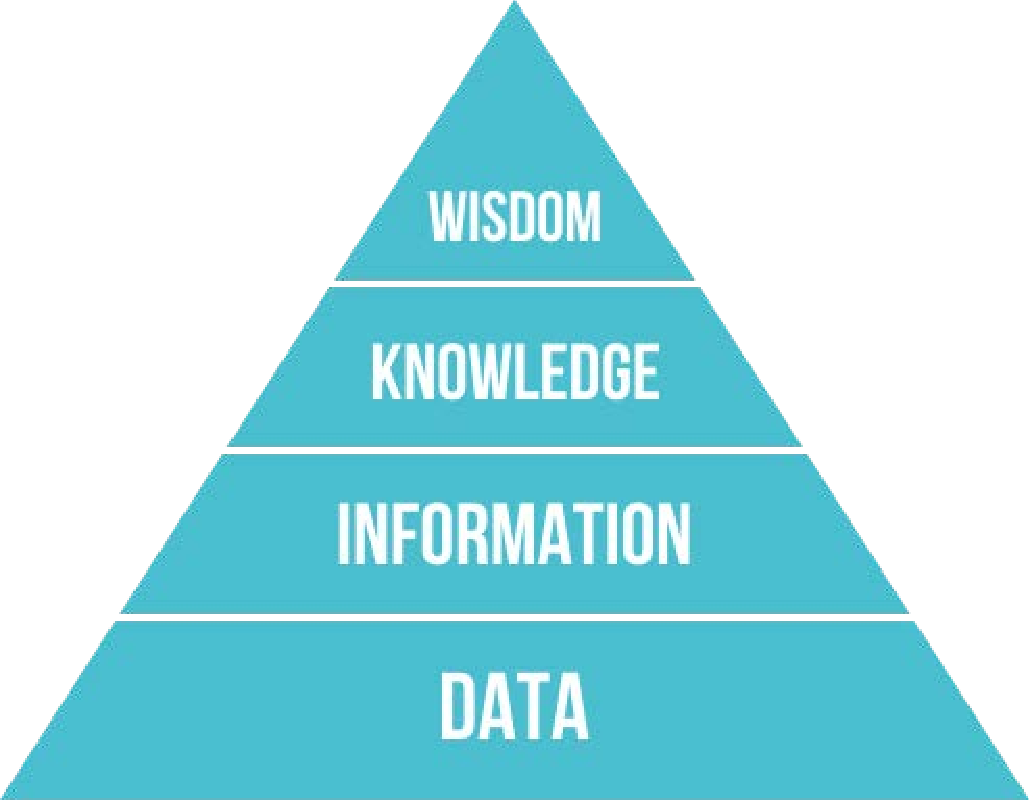
\includegraphics[width=0.30\columnwidth]{images/DIKW_Pyramid}
\caption{DIKW hierarchical model \cite{editor06}.}
\end{figure}

\subsection{Search Engines}

A web search engine is a software system for searching information on the Internet. The search results are generally presented in a line which are often referred to as search engine results pages. And some search engines also haeve the capability to mine data from databases or other open directories. Unlike web directories, which are maintained only by human editors, search engines also maintain web crawling, indexing and searching processes in real-time \cite{editor05}. Table 1 displays the development of search engines and some searching technologies in recent years.
\begin{table*}[htb]
\centering
\begin{tabular}{|c|c|} \hline
\textsf{Year} & \textsf{Events} \\ \hline
1990 & First engine ``Archie'' appeared. \\ \hline
1994 & Original Yahoo was human created catalog. \\ \hline
1995-2000 & The classic information retrieval techniques adapted to HTML. \\ \hline 
1998 & Google founded with its link structure by using the PageRank algorithm. \\ \hline
2000-2005 & Add context, spell check, suggestions, multiple sources. \\ \hline
2005- & Add optimization of complete results, topic analysis of documents, social search. \\ \hline
\end{tabular}
\caption{Search engines development.}
\end{table*}

\subsection{Boolean and Vector Space Models}

After discussed the basic principles and the application of web search, here introduce a model that used to define the search technique. Boolean model and vector model are both retrieval model that can be a description of either the computational process or the human process of retrieval. For a retrieval model, it specifies the details of \cite{editor07}: 
\begin{itemize}
\item Document representation.
\item Query representation.
\item Retrieval function (how to find relevant results).
\item Determines a notion of relevance.
\end{itemize}  

In boolean model, keywords are considered to be either present or absent in a
document and to provide equal evidence with respect to information needs. Queries are boolean expressions of keywords, which connected by AND ($\wedge$), OR ($\vee$), and NOT ($\neg$), including the use of brackets to indicate scope \cite{editor07}. Thus, for the output of this model, the result document should be either relevant or not, and could not give partial matches or a ranking. Although this model is easy to understand and offers a clean formalism, it might become extremely complicated for most of web users in big data.

For vector space model, documents and queries are vectors in a high-dimensional space. Assume $t$ distinct terms remain after preprocessing. Each term ($i$) in a document or query ($j$) is given a real valued weight $w_{ij}$. Therefore, both documents and queries are expressed as t-dimensional vectors \cite{editor07}:
\[d_j=(w_{1j},w_{2j},\cdots,w_{tj})\]
There are some patterns to represent term weight. One is the Term Frequency, which assume that important terms have the higher frequency of occurrence in a document. The following equation define the vector space model.
\[tf(t,d)=
  \begin{cases}
    0, & freq(d,t)=0 \\
    1+\log{freq(d,t)}, & \text{otherwise}
  \end{cases}
\]
While $t$ refers to terms, and $d$ refers to documents. This model straightforward to map everything to a vector and compare their angles. But it is hard to find a good set of basis vectors, a good weighting scheme for terms and a comparison function.

\subsection{Web Crawling}

It is not difficult to extract data from web with the help of algorithms. The input of the algorithm could be a list of URL's visited already and a list of new URL's to visit. Then executes the following steps in a loop:
\begin{enumerate}
\item Fetch URL off list and check if done.
\item If not done, go to web and continue collect.
\item Hand document to document analyzer.
\item Extract all URL's and add to list of new URL's to visit.
\end{enumerate}
The result could be lots of detail of course. Then after fetching from the web, it should do the following steps:
\begin{enumerate}
\item Convert document from HTML, PDF, Word, $\ldots$ to a text document.
\item Tokenization: remove formatting, punctuation, capitals and convert to common form which makes document become a set of canonical tokens.
\item Filtration: remove ``stop words'' (e.g. the, is, a, etc.).
\item Stemming and Normalization: remove inflections and cope with non trivial synonyms.
\end{enumerate}
Then the output are contents in bag of words and final terms are those used to define each dimension of vector space model.

\section{Web Data (Text) Mining}
\subsection{Web Data Analysis Steps}
For the big data which people search from web, it could be very difficult to extract or analyze useful information behind them. Thus, it is necessary to define the following steps to make those data structured or orderly so that people could easily applying other techniques like text mining to analyze them.
\begin{enumerate}
\item Get the digital data from web.
\item Preprocess data into searchable data like words or positions.
\item Form Inverted Index in order to map words to documents.
\item Use algorithm like PageRank to rank relevance of documents.
\item Apply some technologies (e.g. reverse engineering, preventing reverse engineering, etc.) for web advertising.
\item Build the structure of the Internet and its people and pages.
\item Clustering documents into topics.
\item Might utilize Bayes to convert Mathematics of frequency into Mathematics of belief.
\end{enumerate}

\subsection{Link Structure Analysis}
Since link structure has the significant impact to Search Engine Rankings, the PageRank flow and the number of pages that get indexed, it became one of the important factors of SEO (Search Engine Optimization) \cite{editor08}.

Link structure explores the connectivity patterns between web pages that contain the useful information and makes the huge of website’s statistics meaningful. That is to say, mining these big data could help us understand what kind of things that users looking for, what are the hottest categories of a website and which pages are the most popular. Continuous optimization of link structure can eliminate duplicate content and promote popular pages in order to get more pageviews and higher rankings on Search Engine results \cite{editor08}.

An idea of the link structure for web pages is Hubs, which is known as Hubs and Authorities. The concept of this idea is simple: certain web pages served as large directories that were not actually authoritative in the information for users, but have links that led users direct to other authoritative pages \cite{editor09}. Figure 2 shows the structure of Hubs.
\begin{figure}
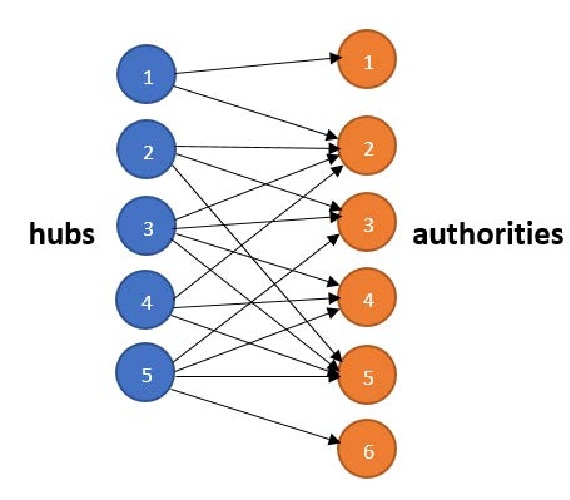
\includegraphics[width=1.0\columnwidth]{images/Hubs_structure}
\caption{Hubs structure for web pages.}
\end{figure}
As it shows in this figure, a good hub represented a page that pointed to many other pages and a good authority represented a page that was linked by many different hubs.

After defined the link structure of web pages, it comes to a link analysis algorithm named PageRank used by Google Search to rank websites in their search engine results. It is a way of measuring the importance of website pages. PageRank assigns a numerical weighting to each element of a hyperlinked set of documents with the purpose of ``measuring'' its relative importance within the set. The numerical weight that it assigns to any given element $E$ is referred to as the PageRank of $E$ and denoted by $PR(E)$ \cite{editor10}. The output of PageRank is a probability distribution that a page will be visited by a person who has the same probability to click each link on this page. This probability could be calculated iteratively with each page getting a contribution at each iteration equal to its page rank divided by the sum of links on page:
\[PR(\text{page } i)=\Sigma_{\text{page } j \text{ pointing at } i}\dfrac{PR(\text{page } j)}{\text{number of pages linked on page } j}\]
For example, a PageRank of 0.5 means there is a 50\% chance that a person clicking on a random link will be directed to the document with the 0.5 PageRank \cite{editor10}. PageRank could be used in ranking academic doctoral programs, recommendation systems and many other searching areas.
    
\subsection{Clustering and Topic Models}
After obtained results through a search query, it is important to classify them by groups for the further analysis. Clustering, also known as grouping document together, is the responses to a search query which give a group of documents. Suppose documents are the points in a space, the task of clustering is to identify regions. There are several ways to do this task:
\begin{itemize}
\item Clustering: Nearby regions of points.
\item Support Vector Machine (SVM): Chop space up into parts.
\item Gaussian Mixture Models (GMMs): A type of fuzzy clustering.
\item K-Nearest Neighbors.
\end{itemize}

Alternatively, some ``hidden meaning'' can be determined with a topic model. It used to discover the abstract "topics" that occur in a collection of documents so that people could group documents by those topics. Topic modeling is a frequently used text-mining tool for discovery of hidden semantic structures in a text body \cite{editor11}. Assume each document is a set of topics and each topic is a bag of words, a topic model aims to find the best set of topics and best set of words in topics through a mathematical framework. That is to say, it allows people to examine a set of documents and discover what the topics might be and what each document's balance of topics is \cite{editor11}.

\section{Conclusion}

The aim of this paper is to demonstrate the core contents and the technique background of web search and text mining in big data area. Since the growth amount of data generate on web everyday cause the traditional computing methods and algorithms inefficiency, it is essential to make innovations in web search aspect. In the recent twenty years, search engines developed quickly and DIKW model, which was known as a popular model used in information system before, has applied in web for building its basic principles as well. As the vector space model appeared, the simple boolean model has been replaced in order to define the search query model more completely. And with the help of web crawling algorithm, multiple types of text data extracted from website have become normalized before mining (analysis) the useful information.

Since webs page could seem as link structure, there must exists some patterns between linked pages. PageRank which found by Google is still widely applied in many different big data systems today, it has the ability to find the most relevant page for the content that the user searches for. After obtained pages of data information, we could utilize clustering to group documents together by topics.

\begin{acks}
The author would like to thank Professor Gregor von Laszewski and all TAs for providing the resource, tutorials and other related materials to write this paper.

\end{acks}

\bibliographystyle{ACM-Reference-Format}
\bibliography{report} 


\end{document}
